\section{Analyse et conception}

\subsection{Données géométriques et constantes}
Les données utilisées proviennent des figures des consignes :
\begin{itemize}
\item Circuit magnétique : \(l_1=\SI{57}{mm}\), \(l_2=\SI{14}{mm}\), \(l_3=\SI{11}{mm}\), \(l_4=\SI{10.5}{mm}\), \(l_5=\SI{18}{mm}\), \(l_6=\SI{6}{mm}\), épaisseur \(e=\SI{15}{mm}\).
\item Bobinage primaire : \(N_1=500\), diamètre fil \(d_1=\SI{0.4}{mm}\), dimensions \(l_1'=\SI{17}{mm}\), \(l_2'=\SI{19}{mm}\), \(l_3'=\SI{29}{mm}\), \(l_4'=\SI{32}{mm}\).
\item Bobinage secondaire : \(N_2=200\), diamètre fil \(d_2=\SI{0.2}{mm}\).
\item Cuivre : \(\rho_{20}=\SI{1.724e-8}{\ohm.m}\), \(\alpha=\SI{3.93e-3}{K^{-1}}\).
\end{itemize}

Section d'entrefer efficace (colonne centrale) :
\[
S_g \approx l_3\,e = (\SI{11}{mm})(\SI{15}{mm}) = \SI{165}{mm^2}=\SI{1.65e-4}{m^2}.
\]

\subsection{Résistance de la bobine principale}
La longueur moyenne par spire est estimée à partir du périmètre moyen du rectangle bobiné :
\[
\ell_{\text{spire,moy}}=2\left(\frac{l_1'+l_3'}{2}+\frac{l_2'+l_4'}{2}\right)
=2\left(\frac{17+29}{2}+\frac{19+32}{2}\right)=\SI{97}{mm}.
\]
Longueur totale de cuivre :
\[
L_{cu,1}=N_1\,\ell_{\text{spire,moy}}=500\times \SI{97}{mm}=\SI{48.5}{m}.
\]
Section du fil primaire :
\[
A_{cu,1}=\frac{\pi d_1^2}{4}=\frac{\pi(\SI{0.4}{mm})^2}{4}\approx\SI{0.1257}{mm^2}=\SI{1.257e-7}{m^2}.
\]
Résistance à \SI{20}{\degreeCelsius} :
\[
R_1(20)=\rho_{20}\frac{L_{cu,1}}{A_{cu,1}}=1.724\times10^{-8}\times\frac{48.5}{1.257\times10^{-7}}\approx \SI{6.65}{\ohm}.
\]
Variation thermique :
\[
R_1(T)=R_1(20)\bigl[1+\alpha(T-20)\bigr].
\]
\begin{table}[H]
\centering
\caption{Résistance théorique de la bobine primaire}
\begin{tabular}{lccc}
\toprule
Température & \SI{20}{\degreeCelsius} & \SI{100}{\degreeCelsius} & \SI{150}{\degreeCelsius} \\
\midrule
\(R_1(T)\) [\si{\ohm}] & 6.65 & 8.74 & 10.05 \\
\bottomrule
\end{tabular}
\label{tab:R1_theo}
\end{table}

\subsection{Courant de référence (densité de courant imposée)}
Avec \(J=\SI{4.0}{A/mm^2}\) :
\[
I_{\mathrm{ref}}=J\cdot A_{cu,1}=4.0\times 0.1257\approx \SI{0.503}{A}.
\]
On retient \(I_{\mathrm{ref}}\approx\SI{0.50}{A}\).

\subsection{Schéma magnétique équivalent}

\paragraph{Hypothèses.}
Fuites de flux négligées, section uniforme sur chaque branche, flux symétrique dans les deux branches latérales.

La structure double~E comporte \textbf{trois colonnes} séparées par le même entrefer de longueur \(x\) : la colonne centrale (où est bobiné \(N_1\)) et les deux colonnes latérales. Le schéma équivalent est une source de FMM \(\mathcal{F}=N_1I\) en série avec la réluctance de la colonne centrale \(\mathcal{R}_c\), puis en parallèle avec les deux branches latérales \(\mathcal{R}_b\) :
\[
\mathcal{R}_c = \mathcal{R}_{g,c} + \mathcal{R}_{\mathrm{fer},c}, \qquad
\mathcal{R}_b = \mathcal{R}_{g,b} + \mathcal{R}_{\mathrm{fer},b}.
\]

\paragraph{Cas \(\mu_r\to\infty\).}
Toutes les réluctances de fer s'annulent ; seuls les entrefers subsistent. Les trois colonnes ont le même entrefer \(x\) :
\[
\mathcal{R}_{g,c}=\mathcal{R}_{g,b}=\frac{x}{\mu_0 S_g}.
\]
La réluctance équivalente vue par la source de FMM est :
\[
\mathcal{R}_{eq,\infty}
= \mathcal{R}_{g,c}+\frac{\mathcal{R}_{g,b}}{2}
= \frac{x}{\mu_0 S_g}+\frac{x}{2\mu_0 S_g}
= \frac{3x}{2\mu_0 S_g}.
\]

\paragraph{Cas \(\mu_r=400\).}
On regroupe la contribution du fer dans un terme \(\lambda=\ell_{\mathrm{fer,eq}}/\mu_r\) :
\[
\mathcal{R}_{eq,400}
= \frac{3(x+\lambda)}{2\mu_0 S_g}.
\]

\subsection{Hypothèses et domaine de validité}
Le modèle est linéaire de premier ordre. Il est valide si :
\begin{itemize}
\item le matériau n'est pas saturé (\(B\) reste sous le coude de la courbe \(B(H)\)) ;
\item l'hystérèse et les pertes fer sont négligées (valable en quasi-statique) ;
\item les fuites de flux et les effets de franges restent modérés.
\end{itemize}

\subsection{Perméance, flux et induction}
La perméance équivalente est l'inverse de la réluctance :
\[
P_{eq,\infty}=\frac{2\mu_0 S_g}{3x},
\qquad
P_{eq,400}=\frac{2\mu_0 S_g}{3(x+\lambda)}.
\]
Le flux total créé par le primaire est \(\Phi_c=N_1 I\,P_{eq}\). Par symétrie, chaque branche latérale porte \(\Phi_g=\Phi_c/2\). L'induction dans un entrefer latéral vaut :
\[
\boxed{B_\infty(x,I)=\frac{\mu_0 N_1 I}{3x}},
\qquad
\boxed{B_{400}(x,I)=\frac{\mu_0 N_1 I}{3(x+\lambda)}}.
\]
La perméabilité finie du fer revient à augmenter l'entrefer effectif de \(\lambda\). Le champ est supposé uniforme dans l'entrefer (approximation de premier ordre).

\subsection{Courbes théoriques demandées}
On prend \(\lambda=\SI{0.40}{mm}\) (\textit{cf.} comparaison avec les mesures, section~\ref{sec:realisation}).

\begin{figure}[H]
\centering
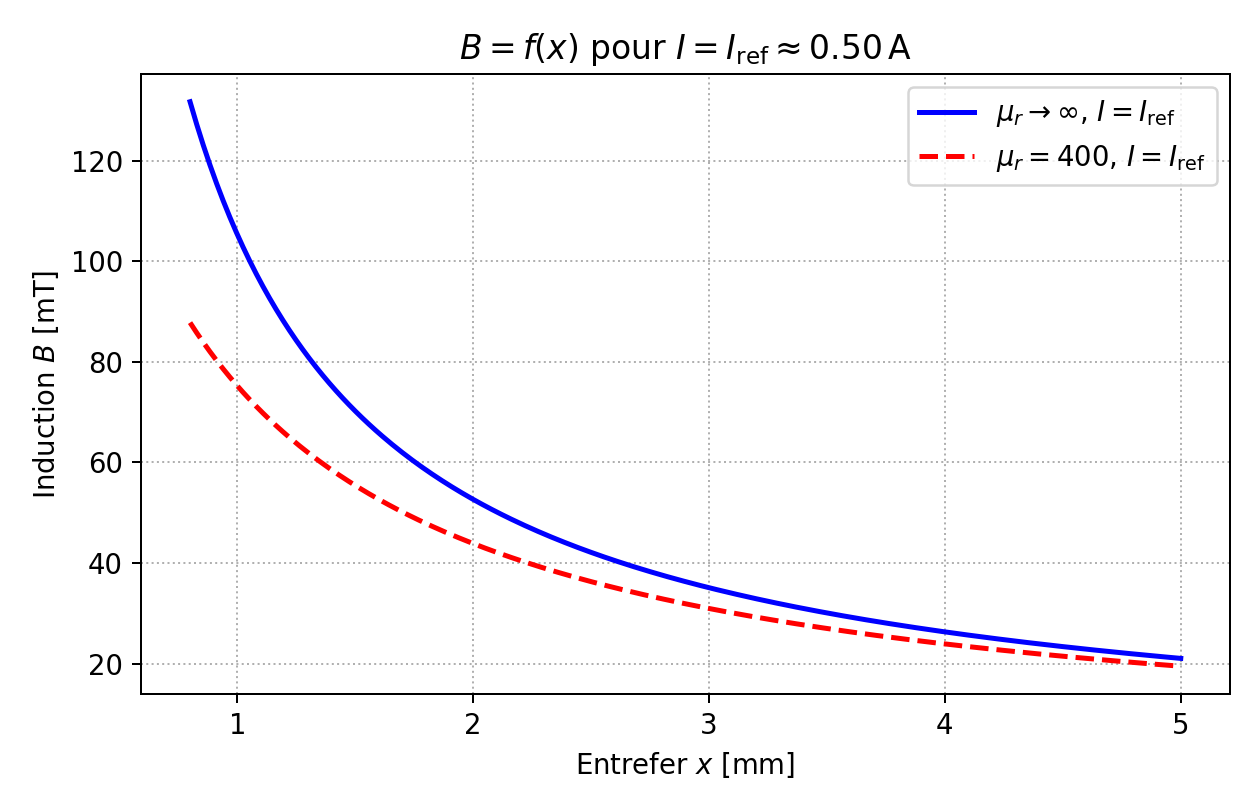
\includegraphics[width=0.85\textwidth]{images/Bfx_theo.png}
\caption{\(B=f(x)\) pour \(I=I_\mathrm{ref}\approx\SI{0.50}{A}\)}
\label{fig:Bfx}
\end{figure}

\begin{figure}[H]
\centering
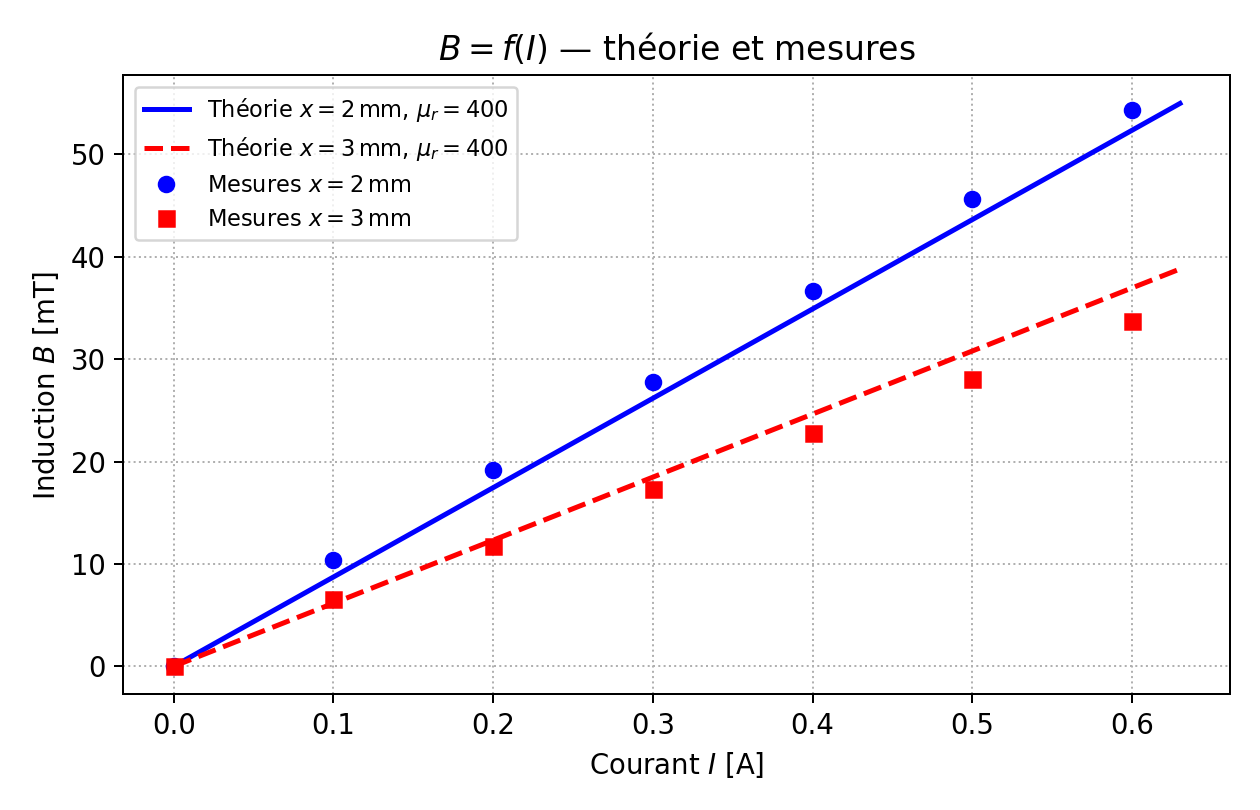
\includegraphics[width=0.85\textwidth]{images/BfI_comp.png}
\caption{\(B=f(I)\) pour \(x=\SI{2}{mm}\) et \(x=\SI{3}{mm}\) — courbes théoriques et points mesurés}
\label{fig:BfI}
\end{figure}

\subsection{Inductances propre et mutuelle}
En négligeant les fuites :
\[
L_{11}(x)=\frac{N_1\,\Phi_c}{I}=\frac{2\mu_0 N_1^2 S_g}{3(x+\lambda)},
\qquad
L_{12}(x)=\frac{N_2\,\Phi_c}{I}=\frac{2\mu_0 N_1 N_2 S_g}{3(x+\lambda)}.
\]
Le rapport \(L_{12}/L_{11}=N_2/N_1=0.4\) est indépendant de \(x\). Pour de petits entrefers, la saturation réduit \(\mu_r\) effectif et fait décroître \(L_{12}\) en dessous de la valeur linéaire.

\begin{table}[H]
\centering
\caption{Valeurs théoriques de référence (\(\lambda=\SI{0.4}{mm}\), \(\mu_r=400\))}
\begin{tabular}{lcc}
\toprule
Entrefer & \(L_{11}\) & \(L_{12}\) \\
\midrule
\(x=0\,\mathrm{mm}\)$^*$ & \(\SI{103}{mH}\) & \(\SI{34.6}{mH}\) \\
\(x=\SI{2}{mm}\)          & \(\SI{14.4}{mH}\) & \(\SI{5.8}{mH}\) \\
\bottomrule
\end{tabular}
\label{tab:L11L12_theo}
\end{table}
\noindent\small$^*$ À $x=0$, le modèle linéaire ($\mu_r=400$ constant) sous-estime fortement $L_{12}$ car la perméabilité réelle du matériau est bien supérieure à 400 à faible induction, et les effets de franges augmentent significativement la perméance effective. La valeur mesurée sera donc significativement supérieure à \SI{34.6}{mH}.

\begin{figure}[H]
\centering
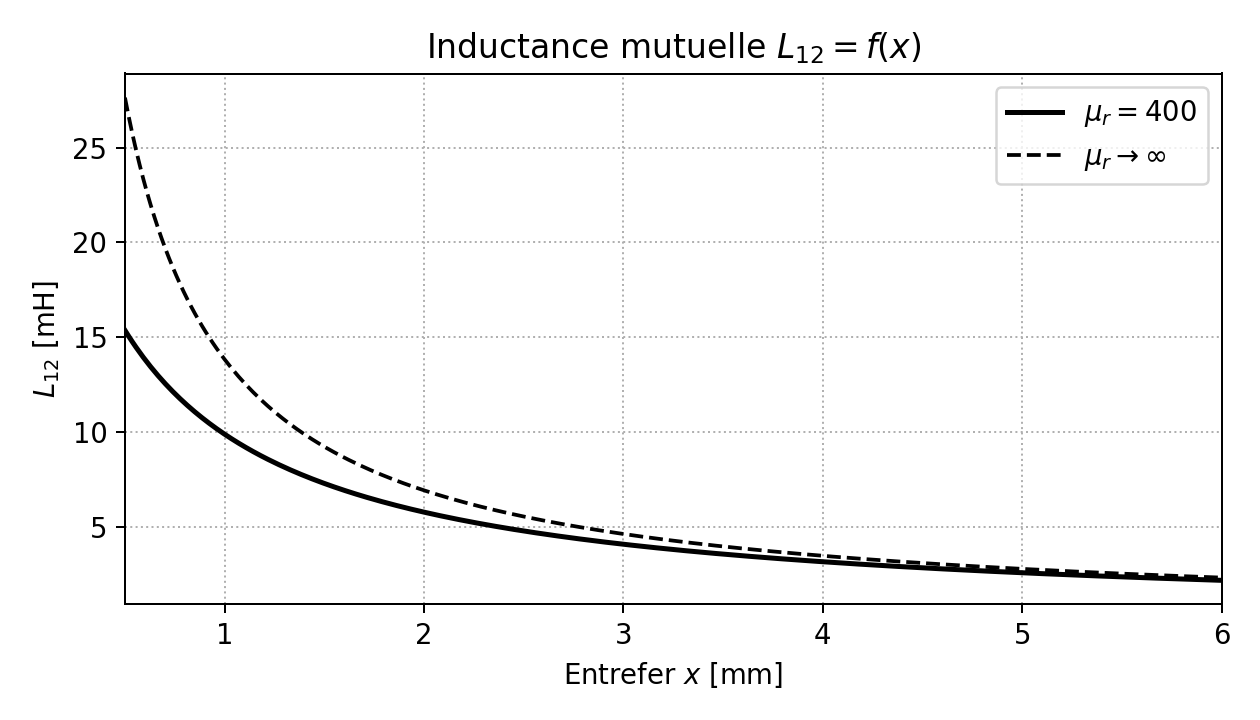
\includegraphics[width=0.85\textwidth]{images/L12fx.png}
\caption{Caractéristique théorique \(L_{12}=f(x)\)}
\label{fig:L12fx}
\end{figure}

\subsection{Bobine secondaire en régime alternatif}
\label{sec:BobSecAC}
L'impédance du primaire (secondaire en circuit ouvert) est :
\[
Z_1=R_1+j\omega L_{11}, \qquad I_1=\frac{U_1}{R_1+j\omega L_{11}}.
\]
Le flux totalisé dans le secondaire est \(\Psi_2=L_{12}I_1\) ; la tension induite vaut :
\[
U_2=j\omega L_{12}I_1=j\omega L_{12}\frac{U_1}{R_1+j\omega L_{11}}.
\]
Cas limites :
\begin{itemize}
\item \(\omega L_{11}\gg R_1\) (régime inductif) :
  \(I_1\approx U_1/(j\omega L_{11})\),\quad
  \(U_2\approx \dfrac{L_{12}}{L_{11}}\,U_1= \dfrac{N_2}{N_1}\,U_1\).
\item \(\omega L_{11}\ll R_1\) (régime résistif) :
  \(I_1\approx U_1/R_1\),\quad
  \(U_2\approx j\omega L_{12}U_1/R_1\) (croît avec \(\omega\)).
\end{itemize}
À \SI{35}{Hz}, avec \(L_{11}\approx\SI{10}{mH}\) et \(R_1\approx\SI{6.65}{\ohm}\) : \(\omega L_{11}/R_1\approx0.33\). Le primaire est dans un régime intermédiaire.

Le flux se reconstruit par intégration de la tension secondaire :
\[
\Psi_2(t)=\int_0^t U_2(\tau)\,d\tau.
\]
